% coding:utf-8

%FOSASTOC, a LaTeX-Code for a electrical summary of stochastic
%Copyright (C) 2013, Daniel Winz, Ervin Mazlagic

%This program is free software; you can redistribute it and/or
%modify it under the terms of the GNU General Public License
%as published by the Free Software Foundation; either version 2
%of the License, or (at your option) any later version.

%This program is distributed in the hope that it will be useful,
%but WITHOUT ANY WARRANTY; without even the implied warranty of
%MERCHANTABILITY or FITNESS FOR A PARTICULAR PURPOSE.  See the
%GNU General Public License for more details.
%----------------------------------------

\chapter{Statistischer Test}
Statistische Tests oder auch \emph{Hypothesentests} werden angewandt um
gemachte Beobachtungen mit einer statistischen Verteilung zu vergleichen.

Die Durchführung und Qualität eines solchen Tests hängt von vielen Faktoren
ab und kennt auch einige Methoden zur Überprüfung und Bewertung der
getroffenen Entscheidungen.

\newpage
\section{Vorgehen}
Bei der Durchführung eines Hypothesentests kann stets nach folgendem Ablauf 
vorgegangen werden.

\begin{enumerate}
	\item Modellwahl \\ 
		\textit{Mit welcher Verteilung sollen die Daten verglichen 
			werden?}
	\item Nullhypothese formuleiren \\
		\textit{Welche Hypothese soll mittels der Daten verworfen 
			werden?}
	\item Alternativhypothese \\
		\textit{Welche Hypothese soll der Test bekräftigen?}
	\item Teststatistik erstellen \\
		\textit{Teststatistik aus dem gewählten Modell und der 
			Nullhypothese erstellen.}
	\item Signifikanzniveau wählen \\
		\textit{Mit welcher Signifikanz soll der Test durchgeführt 
			werden?}
	\item Verwerfungsbereich berechnen \\
		\textit{Aus der Teststatistik und dem gewählten 
			Signifikanzniveau wird der Verwerfungsbereich 
			berechnet (oder einfach der P-Wert verwendet).}
	\item Testentscheid \\
		\textit{Daten werden mit dem berechneten Verwerfungsbereich 
			(oder dem P-Wert) verglichen und basierend darauf ein 
			Entscheid gefällt}
\end{enumerate}

\section{Konfidenzintervall}
Das Konfidenzintervall (auch \emph{Vertrauensintervall} oder 
\emph{Mutungsintervall}) beschreibt einen Bereich einer Verteilung.
Liegen Beobachtungen innerhalb dieses Bereiches, so vertraut man auf
deren Gültigkeit. Im Umfeld von statistischen Tests wird alles 
ausserhalb des Konfidenzintervalls als Verwerfungsbereich
benannt.

\begin{figure}[h!]
	\centering
	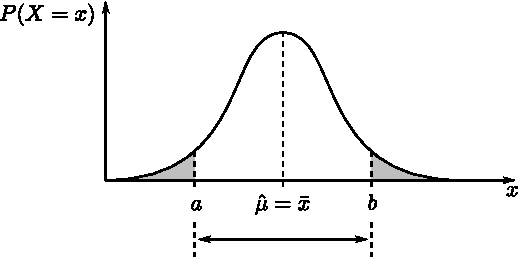
\includegraphics[width=0.7\textwidth]{konfidenzintervall.pdf}
	\caption{Konfidenzintervall}
	\label{fig:konfidenzintervall}
\end{figure}

Die Intervallgrenzen werden durch kummulative Wahrscheinlichkeitswerte
bzw. Quantile gebildet, welche durch die gewählte Genaugkeit bestimmt 
werden. Die Intervallgrenzen werden oft auch mittels des sog. 
Signifikanzniveaus $\alpha$ beschrieben, was nichts weiter ist als die 
Differenz aus $1$ und der Genauigkeit $g$.
\[ \begin{array}{l c l} 
	P(a \leq \mu \leq b) = g 
		& 
		& 0 \leq g \leq 1, \quad \alpha = 1-g \\
	& & \\
	 a = \displaystyle q\left(\frac{1-g}{2}\right) 
			= q\left( \frac{\alpha}{2} \right)
		&
		&\\
	& & \\
	b = \displaystyle q\left(1-\frac{1-g}{2}\right) 
			= q\left(1-\frac{\alpha}{2}\right) 
		&
		&\\
\end{array} \]
Die Grenzen des Intervalls müssen nicht zwingend symmetrisch liegen, 
denn es kann auch ein sog. einseitiger Test erfolgen. Bei einem 
einseitigen Test gibt es nur einen geschlossenen Verwerfungsbereich
welcher passenderweise mit dem Signifikanzniveau beschrieben wird.

\section{P-Wert}\label{sec:p-wert}
Der P-Wert (engl. \emph{p-Value}) ist ein Wert, welcher die kummulative 
Wahrscheinlichkeit abbildet vom Punkt der Beobachtung aufwärts. D.h.
der P-Wert beschreibt die Wahrscheinlichkeit die gemachte Beobachtung 
oder extremere Beobachtungen zu erhalten.

\begin{figure}[h!]
	\centering
	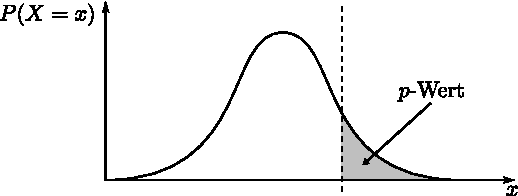
\includegraphics[width=0.7\textwidth]{p-value.pdf}
	\caption{P-Wert graphisch dargestellt}
	\label{fig:p-wert}
\end{figure}

\subsection{Interpretation}
Der P-Wert eignet sich um das Berechnen des Verwerfungsbereiches auszulassen,
denn man kann anhand des P-Wertes und des Signifikanzniveaus direkt den 
Entscheid für einen einseitigen Test fällen.

\[ 
	\begin{array}{c c l}
		p\text{-Wert} > (1-\alpha)
			& \Rightarrow
			& \text{Hypothese nicht verwerfen} \\
		& & \\
		p\text{-Wert} < (1-\alpha)
			& \Rightarrow
			& \text{Hypothese verwerfen}
	\end{array} 
\]

\section{Fehler}
Die Ausführung eines statistischen Tests bzw. eines Hypothesentests bedingt,
dass ein Entscheid gefällt wird über die Nullhypothese. Diese kann entweder
beibehalten oder verworfen werden. Jede der gemachten Entscheidungen kann dabei
zwei Auswirkungen aufweisen welche in der Tabelle \ref{tab:wirkungstabelle} 
dargestellt sind.

\begin{table}[h!]
	\centering
	\begin{tabular}{l c c}
		Entscheidung
			& $H_0$ ist wahr 
			& $H_0$ ist falsch \\
		\hline
		&& \\
		$H_0$ beibehalten 
			& korrekt 
			& Fehler 2. Art \\
		&& \\
		$H_0$ verworfen 
			& Fehler 1. Art 
			& korrekt \\
		&& \\
	\end{tabular}
	\caption{Wirkungstabelle von Hypothesentests}
	\label{tab:wirkungstabelle}
\end{table}

Unabhängig von den Ursachen eines falschen Entscheides muss dieser 
berücksichtigt werden. Die zwei auftretenden Fehler werden als
Fehler 1. bzw. Fehler 2. Art bezeichnet.

\subsection{Fehler 1. Art}
Der Fehler 1. Art tritt ein, wenn die Nullhypothese verworfen wird, obwohl 
sie wahr ist. 

\begin{figure}[h!]
	\centering
        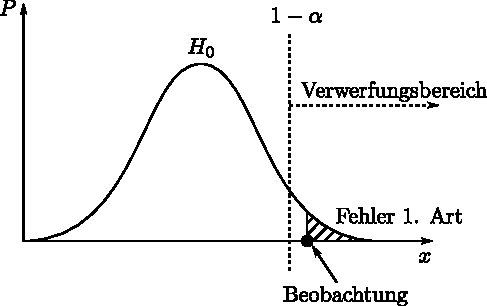
\includegraphics[width=0.7\textwidth]{fehler-erster-art.pdf}
	\caption{Fehler 1. Art}
	\label{fig:fehler1}
\end{figure}

Er beschreibt die Summe aller Wahrscheinlichkeiten die extremer als die 
gemachte Beobachtung sind (siehe P-Wert, Kapitel \ref{sec:p-wert}). 
Der Fehler 1. Art ist somit limitiert auf den Wert des Signifikanzniveaus 
$\alpha$, denn wenn der Wert für den Fehler 1. Art grösser wäre, so müsste 
er ausserhalb des Verwerfungsbereiches liegen und die die Hypothese konnte 
gar nicht verworfen werden.

\subsection{Fehler 2. Art}
Der Fehler 2. Art tritt ein, wenn die Nullhypothese nicht verworfen wird, 
obwohl sie falsch ist bzw. die Alternative wahr ist.

\begin{figure}[h!]
	\centering
	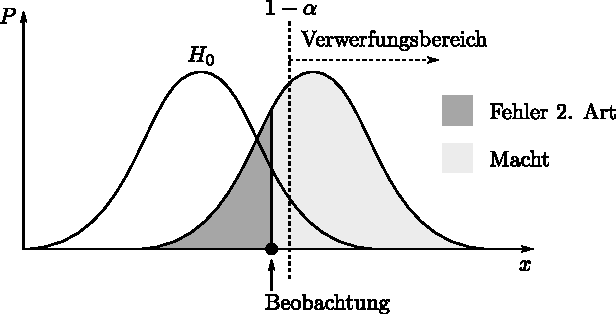
\includegraphics[width=0.85\textwidth]{fehler-zweiter-art.pdf}
	\caption{Fehler 2. Art}
	\label{fig:fehler2}
\end{figure}

Um den Fehler 2. Art zu berechnen, muss eine alternative Verteilung 
explizit (quantitativ) gegeben sein oder angenommen werden. Eine Relation
der Verteilungen ($p_a > p_0$, $p_a < p_0$, $p_a \neq p_0$), welche 
häufig für Hypothesentests angewendet werden, reicht somit nicht aus für
die Berechnung.

\subsection{Macht}
Die sog. Macht gibt Auskunft darüber, wie Aussagekräftig die gemachte
Annahme ist. Der Fehler 2. Art ist die Summe aller Wahrscheinlichkeiten
der alternativen Verteilung, welche weniger extrem als die gemachte 
Beobachtung sind. Die Macht entspricht somit der Differenz von 1 und 
dem Fehler 2. Art.
\[  
	\text{Macht} = 1 - P(\text{Fehler 2. Art})
\]

\clearpage
\newpage
\section{Modellauswahl}
Die richtige Modellauswahl ist bei der Durchführung eines statistischen
Tests von entscheidender Bedeutung. Eine einfache Entscheidungsvorschrift
ist in der Grafik \ref{fig:modellauswahl} gegeben.

\tikzstyle{decision} = [diamond, 
			draw, 
			fill=gray!20, 
			text width=5.0em, 
			text badly centered, 
			%node distance=3cm, 
			inner sep=0pt]

\tikzstyle{block} = [	rectangle, 
			draw, 
			fill=gray!20, 
			text width=5.0em, 
			text centered, 
			rounded corners,
			%node distance=3cm,
			inner sep=0pt,
			minimum height=4em]

\tikzstyle{line} = [	draw, 
			-latex']

\tikzstyle{cloud} = [	draw, 
			ellipse,
			fill=gray!20, 
			%node distance=3cm,
			minimum height=2em]

\begin{figure}[h!]
	\centering
	\begin{tikzpicture}[auto, scale=0.85, every node/.style={scale=0.85}]
		% nodes
		\node [block] 		at ( 5,14) 	(start) 	{Test};
		\node [decision] 	at ( 5,11)	(bernoulli?) 	{Bernoulli?};
		\node [decision] 	at ( 2, 8)	(offen?) 	{nach oben offen?};
		\node [block] 		at ( 2, 2)	(poisson) 	{Poisson Test};
		\node [block] 		at ( 4, 2)	(binom)		{Binomial Test};
		\node [decision]	at ( 9, 8)	(normal?)	{Normal verteilt?};
		\node [block]		at ( 6, 2)	(z)		{z Test};
		\node [decision]	at ( 6, 5)	(std?)		{$\sigma$ bekannt?};
		\node [block]		at ( 8, 2)	(t)		{t Test};
		\node [decision]	at (12, 5)	(symmetrie?)	{Symmetrie?};
		\node [block]		at (10, 2)	(wilcox)	{Wilcoxon Test};
		\node [block]		at (12, 2)	(vorzeichen)	{Vorzeichen Test};
%		% paths
		\path [line] (start) 		-- (bernoulli?);
		\path [line] (bernoulli?) 	-| node [near start] {ja} (offen?);
		\path [line] (bernoulli?)	-| node [near start] {nein} (normal?);
		\path [line] (offen?)		-- node [near start] {ja} (poisson);
		\path [line] (offen?)		-| node [near start] {nein} (binom);
		\path [line] (normal?)		-| node [near start] {ja} (std?);
		\path [line] (normal?)		-| node [near start] {nein} (symmetrie?);
		\path [line] (std?)		-- node [near start] {ja} (z);
		\path [line] (std?)		-| node [near start] {nein} (t);
		\path [line] (symmetrie?)	-| node [near start] {ja} (wilcox);
		\path [line] (symmetrie?)	-- node [near start] {nein} (vorzeichen);
	\end{tikzpicture}
	\caption{Vorschrift zur Modellauswahl als Flussdiagramm}
	\label{fig:modellauswahl}
\end{figure}

\subsection{Entscheidungshilfen}

\paragraph{Bernoulli?}
Beschreiben die Daten eine Reihe von unabhängigen 
Bernullientscheiden (binär)?

Typisches Beispiele: Münzwurf, Würfelspiel.

\paragraph{nach oben offen?}
Sind die Daten solche, welche keine (theoretische) obere Grenze kennen?

Typische Beispiele: Anzahl Anrufe eines CallCenters, Anzahl Requests auf 
einen Server .

\paragraph{Normal verteilt?}
Lassen sich die Daten als Noralverteilung betrachten 
(z.B. mittels eines QQ-Norm Plots)?

Typische Beispiele: Körpergrössen einer grossen Personengruppe,
Abfüllmengen, Bauteilwerte (z.B. Widerstandwert). 

\paragraph{$\sigma$ bekannt?}
Ist die Standardabweichung $\sigma$ bekannt?

\paragraph{Symmetrie?}
Sind die Daten symmetrisch um einen Punkt $x$ verteilt?


\newpage
\section{Binomial-Test}
Der Binomial-Test ist immer dann anzuwenden, wenn eine 
Binomialverteilung vorliegt. Dieser Test kann ein- oder zweiseitig
durchgeführt werden, d.h. das Signifikanzniveau wird entweder von
unten, oben oder geteilt auf beide Seiten gesetzt (nur symmetrisch
wenn auch die Verteilung symmetrisch ist). 

\subsection{Formales Vorgehen}

\begin{table}[h!]
	\begin{tabular}{l l}
		Modell 
			& $X \sim Bin(n,p)$ \\
		& \\
		Nullhypothese
			& $H_0: p_0 = \mu_0$ \\
		& \\
		Alternativhypothese 
			& $H_A: p_A > p_0 = \mu_0$ \\
			& $H_A: p_A \neq p_0 = \mu_0$ \\ 
			& $H_A: p_A < p_0 = \mu_0$ \\
		& \\
		Teststatistik
			& $X: P(X=x|H_0) = \binom{n}{x} {p_0}^x (1-p_0)^{n-x}$ \\
		& \\
		Signifikanzniveau
			& $\alpha$ \\
		& \\
		Verwerfungsbereich
			& \\
		~~~~~beidseitig
			& $K_b = \left(\left[
					0,q\left(\frac{\alpha}{2}\right)
				\right] \cup 
				\left[
					q\left(\frac{\alpha}{2}\right),1
				\right]\right)$ \\ 
		~~~~~links
			& $K_l = \left(\left[
					0, a = q\left(\alpha
				\right)\right]\right)$ \\
		~~~~~rechts
			& $K_r = \left(\left[ 
					q\left(\alpha\right),1
				\right]\right)$ \\
		& \\
		Testentscheid
			& \\
		~~~~~$X \in K$
			& Nullhypothese wird verworfen \\
		~~~~~$X \not\in K$
			& Nullhypothese wird beibehalten \\ 
	\end{tabular}
	\caption{Formales Vorgehen des Binomial-Test}
\end{table}

\subsection{\lstinline{binom.test()}}
In R lässt sich ein Binomial-Test mit der Funktion 
\lstinline{test.binom()} ausführen. Hierbei gilt es die Parameter
zu beachten.

\begin{Schunk}
\begin{Sinput}
> hits <- 39 # number of successes
> trials <- 215 # number of trials
> prob <- 0.15 # hypothesized probability of success
> binom.test(x=hits, n=trials, p=prob, alternative="less", conf.level=0.95)
\end{Sinput}
\begin{Soutput}
	Exact binomial test

data:  hits and trials
number of successes = 39, number of trials = 215, p-value = 0.9142
alternative hypothesis: true probability of success is less than 0.15
95 percent confidence interval:
 0.000000 0.230171
sample estimates:
probability of success 
             0.1813953 
\end{Soutput}
\end{Schunk}

\section{Poisson-Test}
\section{z-Test}
\section{t-Test}
\section{Wilcoxon-Test}
\section{Vorzeichen-Test}
